\chapter{An Introduction to the Standard Model and Top Quark Physics}\label{chapter:theory}
\section{The Standard Model}\label{sec:sm}
The Standard Model (SM) of particle physics describes all the known elementary matter particles and their interactions with the weak, strong, and electromagnetic forces using renormalisable Quantum Field Theory (QFT).
QFT describes particles as excitations of quantum fields, whose dynamics are typically described using the Lagrangian formalism~\cite{LagrangiansSM}.

This chapter introduces and briefly describes the theoretical framework of the SM, the shortcomings of the SM and the physics of the top quark.
The second section of the chapter discusses the motivations and context of the search for a single top quark produced in association with a Z boson presented in this thesis.

Throughout this thesis \emph{natural units}, where the fundamental constants $c$, $\hbar$ and $k_{B}$ (Boltzmann constant) are set to unity, and Einstein's summation convention are used.

\subsection{Fundamental Particles}\label{subsec:particles}
The SM describes all matter as being made up of spin-$\frac{1}{2}$ particles known as fermions that interact through the fundamental forces, which are mediated by spin-$1$ gauge bosons.
The spin-$0$ Higgs boson arises as a consequence of the breaking of the electroweak symmetry,  imbuing the massive weak force gauge bosons with mass and providing an explanation for how fermions acquire their mass .

Matter consists of six quarks, fundamental particles that interact through the strong, electromagnetic and weak forces, and six leptons, fundamental particles that do not experience the strong force~\cite{LagrangiansSM}.
Each fermion has an associated anti-matter equivalent, which has identical mass but opposite charge.
Both types of fermion are subdivided into three ``generations'' of particles where each subsequent generation of particles is identical, except for their quantum number and mass~\cite{ElectroweakStrong}.
Table~\ref{tab:fermions} lists the charges, weak isospins and masses of the quarks and leptons for each of the three generations.

The ``up-type'' and ``down-type'' quarks have an electrical charges of $+\frac{2}{3}$ and $-\frac{1}{3}$,  respectively, and \emph{colour charges} (or anti-colour charges) of red, blue or green.
As the phenomena of \emph{colour confinement} (described in Section~\ref{subsec:QCD}) only allows for colourless states, quarks form composite particles collectively called hadrons.
Typically hadrons are composed of a quark anti-quark pair, known as mesons, or of groups of three quarks, referred to as baryons.
Exotic hadrons formed of larger groupings of quarks can be also formed, with both tetraquark and pentaquark states having been observed by the LHCb detector~\cite{Aaij:2014jqa,Aaij:2015tga} and elsewhere~\cite{Tanabashi:2018oca}.

Each generation of leptons consists of a charged lepton that interacts through the electromagnetic and weak forces, and a corresponding neutral near massless lepton, known as a neutrino, that interacts solely through the weak force.
As with the quarks, the charged lepton of each subsequent generation is more massive than the last.
Initially, it was assumed that neutrinos were massless, but the discovery of neutrino flavour oscillation implies that they must have non-zero masses. 
The hierarchy of the neutrino mass eigenstates is currently unknown~\cite{Nath:2018rqn}.

\begin{table}[htbp]
\topcaption {
The Standard Model fermions and their properties~\cite{Tanabashi:2018oca}.
}
\label{tab:fermions}
  \centering
  \resizebox{\textwidth}{!}{
% This right-aligns numbers in column, but centers them under column title.
 \begin{tabular}{llllccc}
   \hline
   & \textbf{Generation} & \textbf{Particle} & \textbf{Mass [\MeV]} & \textbf{Electric Charge} & \textbf{Weak Isospin}\\
   \hline
   \multirow{3}{*}{Quarks}  & \multirow{2}{*}{I} & up (\textit{$u$})  & $2.2^{+0.5}_{-0.4}$ & $+ \frac{2}{3}$ & $+ \frac{1}{2}$ \\
   & & down (\textit{$d$}) & $4.8^{+0.5}_{-0.3}$ & $- \frac{1}{3}$ & $- \frac{1}{2}$ \\
   & \multirow{2}{*}{II} & charm (\textit{$c$})  & $1.275^{+0.025}_{-0.035} \times 10^{3}$ & $+ \frac{2}{3}$ & $+ \frac{1}{2}$ \\
   & & strange (\textit{$s$})  & $95^{+9}_{-3}$	 & $- \frac{1}{3}$ & $- \frac{1}{2}$ \\
   & \multirow{2}{*}{II} & top (\textit{$t$})  & $(173.1 \pm 0.9) \times 10^{3}$ & $+ \frac{2}{3}$ & $+ \frac{1}{2}$ \\
   & & bottom (\textit{$b$})  & $(4.18^{+0.04}_{0.03}) \times 10^{3}$ & $- \frac{1}{3}$ & $- \frac{1}{2}$ \\
   \hline
   \multirow{3}{*}{Leptons}  & \multirow{2}{*}{I} & electron (\textit{$e$})  & $0.511$ & $-1$ & $- \frac{1}{2}$ \\
   & & electron neutrino (\textit{$\nu_{e}$})  & $< 2 \times 10^{-6}$ & $0$ & $+ \frac{1}{2}$ \\
   & \multirow{2}{*}{II} & muon (\textit{$\mu$})  & $106$ & $-1$ &  $-\frac{1}{2}$ \\
   & & muon neutrino (\textit{$\nu_{\mu}$})  & $< 0.19$ & $0$ & $+ \frac{1}{2}$ \\
   & \multirow{2}{*}{II} & tau (\textit{$\tau$})  & $1777$ & $0$ & $- \frac{1}{2}$ \\
   & & tau neutrino (\textit{$\nu_{\tau}$})  & $<18.2$ & $0$ & $+ \frac{1}{2}$ \\   
   \hline   
 \end{tabular}}
\end{table}

The SM contains five integer spin gauge bosons, shown in table~\ref{tab:bosons}, along with their corresponding masses, charges, and weak isospins.
The four spin-$1$ vector bosons mediate the electromagnetic, weak and strong forces.
The massless photon, $\gamma$, mediates the electromagnetic force, while the massive neutral $Z^0$ and charged  $W^\pm$ bosons mediate the weak force.
Massless gluons mediate the strong force and have one of eight colour states~\cite{LagrangiansSM}. 
The spin-$0$ Higgs boson accounts for fundamental particles acquiring mass.

\begin{table}[htbp]
\topcaption {
The fundamental forces of nature and the SM bosons which mediate them~\cite{Tanabashi:2018oca}.
}
\label{tab:bosons}
  \centering
  \resizebox{\textwidth}{!}{
% This right-aligns numbers in column, but centers them under column title.
 \begin{tabular}{lcccc}
   \hline
   Bosons & Mass [\GeV] & Electrical Charge & Colour Charge & Weak Isospin \\
   \hline
   Photon ($\gamma$) & $0$ & $0$ & $0$ & $0$ \\
   \hline
   W ($\text{W}^{\pm}$) & $80.385 \pm 0.015$ & $\pm 1$ & $0$ & $\pm 1$ \\
   Z ($\text{Z}^0$) & $91.1876 \pm 0.0021$ & $0$ & $0$ & $0$ \\
   Higgs ($\text{h}^{0}$) & $125 \pm 0.24$ & $0$ & $0$ & $- \frac{1}{2}$ \\
   \hline
   \multirow{2}{*}{Gluon ($g$)} & \multirow{2}{*}{$0$} & \multirow{2}{*}{$0$} & $r \overline{g}$, $r \overline{b}, g \overline{r}, g \overline{b}, b \overline{r}, b \overline{g} $ & \multirow{2}{*}{$0$}  \\
   & & &  $\frac{1}{\sqrt{2}}(r \overline{r} - g \overline{g}), \frac{1}{\sqrt{6}}(r \overline{r} + g \overline{g} - 2 b \overline{b})$ & \\
   \hline   
 \end{tabular}}
\end{table}	

\subsection{Gauge Symmetries}\label{subsec:gaugeSymmetries}
The idea that the laws of physics are consistent for all observers, even if the measurements differ between observers, is a fundamental component of all modern physical theories~\cite{Haywood}.
Systems that are unchanged or \emph{invariant} under a given transformation are considered to possess a corresponding \emph{symmetry}.

As shown by Noether's theorem, the generator(s) of any such symmetry conserve a corresponding quantity~\cite{Noether:1918zz}.
Examples of such quantities include the conservation of energy-momentum from space-time symmetry or electrical charge from the $U(1)$ symmetry in electromagnetism.
If a symmetry transformation has no space-time dependence it is said to have a \emph{global symmetry} and conversely, if it has a space-time dependence it is said to have a \emph{local} or \emph{gauge symmetry}~\cite{Cheng:1985bj}.

These concepts can be demonstrated by considering applying the $U(1)$ gauge symmetry of Quantum Electrodyanmics, the theory of electromagnetism, to the Lagrangian of a relativistic spin-$\frac{1}{2}$ free-fermion field (\eg electrons) with a wavefunction $\psi(x)$ and mass $m$~\cite{QFT}:

\begin{equation}
\mathcal{L} = \bar{\psi}(x) (i {\gamma}^{\mu} \partial_{\mu} - m) \psi(x) \;
\label{eq:diracLagrangian}
\end{equation}

where $\partial_{\mu}$ is the partial derivative operator ${\gamma}^{\mu}$ are the Dirac matrices, defined in Appendix~\ref{app:maths}.

If we consider this Lagrangian to have a global $U(1)$ symmetry, then $\psi(x)$ transforms as:

\begin{equation}
\psi(x) \rightarrow \psi'(x) = e^{-i q \alpha} \psi(x) \\
\label{eq:globalTransformation}
\end{equation}

which leaves the Lagrangian in Equation~(\ref{eq:diracLagrangian}) unchanged as $q$ is a constant and $\alpha$ is an arbitrary phase.

If Equation~(\ref{eq:diracLagrangian}) has a local $U(1)$ symmetry, then $\psi(x)$ transforms according to:

\begin{equation}
\psi(x) \rightarrow \psi'(x) = \psi(x) e^{-i q \alpha (x) } \;
\label{eq:localTransformation}
\end{equation}

As such a local transformation involves $\alpha$ being dependent on $x$, the derivative term in Equation~(\ref{eq:diracLagrangian}) now transforms as:

\begin{equation}
\begin{split}
\bar{\psi}(x) \partial_{\mu} \psi(x) \rightarrow \bar{\psi}'(x) \partial_{\mu} \psi'(x) &= \bar{\psi} (x) e^{i q \alpha (x) } \partial_{\mu} \big(e^{-i q \alpha (x) } \psi(x) \big) \\
&= \bar{\psi} (x) \partial_{\mu} \psi(x) - i \bar{\psi} (x) \partial_{\mu} \alpha (x) \psi(x) \\
\end{split}
\label{eq:derivativeLocalTransformation}
\end{equation}

which consequently results in the Lagrangian no longer being invariant:

\begin{equation}
\mathcal{L} \rightarrow \mathcal{L}' = \mathcal{L} + \bar{\psi}(x) \big( i {\gamma}^{\mu} \partial_{\mu} \alpha(x) \big) \psi(x) \;
\label{eq:localLagrangian}
\end{equation}

For the Lagrangian to remain invariant under local transformations, a vector or \emph{gauge} field, $A_{\mu}(x)$, associated with the $\psi(x)$ field, can be introduced, which transforms as follows:

\begin{equation}
A_{\mu}(x) \rightarrow A_{\mu}(x)' + \frac{1}{q} \partial_{\mu} \alpha(x) \;
\label{eq:vectorField}
\end{equation}

This field can be simply introduced by replacing the derivative $\partial_{\mu}$ with the \emph{gauge covariant derivative}~\cite{QFT}, which is defined as $D_{\mu} = \partial_{\mu} - i A_{\mu}(x)$.
As $D_{\mu}$ transforms as:

\begin{equation}
D_{\mu}\psi(x) \rightarrow e^{-i q \alpha (x) } D_{\mu} \psi(x) \;
\label{eq:Dtransform}
\end{equation}

the non-invariant term in Equation~(\ref{eq:localLagrangian}) cancels out and ensures that the Lagrangian remains invariant under the local $U(1)$ gauge transformations.

The presence of this gauge field allows for the inclusion of a gauge invariant term containing a field strength tensor $F_{\mu \nu}$, that describes the geometry of $A_{\mu}(x)$, in the Lagrangian.
The general form of $F_{\mu \nu}$ is given by:

\begin{equation}
F^{a}_{\mu \nu} = \partial_{\mu} A^{a}_{\nu} - \partial_{\nu} A^{a}_{\mu} + g f^{abc} A^{b}_{\mu} A^{c}_{\nu} \;
\label{eq:fieldStrengthTensor}
\end{equation}

where $g$ is the self-coupling constant and $f^{abc}$ are the structure constants of the symmetry group.

For the case of QED, as $U(1)$ has only one generator, which self-commutes, $g$ is zero.

Therefore, with the addition of the simplest gauge invariant term for incorporating $F_{\mu \nu}$, the QED Lagrangian is given by:

\begin{equation}
\mathcal{L}_{QED} = \bar{\psi} (i {\gamma}^{\mu} D_{\mu} - m) \psi - \frac{1}{4} F_{\mu \nu} F^{\mu \nu} \;
\label{eq:qedLagrangian}
\end{equation}

where excitations of the gauge field $A_{\mu}$ correspond to the massless photon and $q$ represents the electric charge of the electron. 

Similarly, by requiring the SM Lagrangian to be gauge invariant under the $SU(3)_{C}$ gauge symmetry of the strong force and under the $SU(2)_{L} \times U(1)_{Y}$ gauge symmetry of the electroweak force, the gauge fields and their associated gauge bosons for the electromagnetic, weak and strong forces naturally emerge.

The resultant SM Lagrangian is constructed of four terms:

\begin{equation}
\mathcal{L}_{SM} = \mathcal{L}_{Gauge} + \mathcal{L}_{Fermion} + \mathcal{L}_{Higgs} + \mathcal{L}_{Yukawa} \;
\end{equation}

where $\mathcal{L}_{Gauge}$ describes the spin-$1$ gauge boson fields that arise from requiring that the Lagrangian is invariant under local transformations of the symmetry group and $\mathcal{L}_{Fermion}$ describes the fermion fields.
The $\mathcal{L}_{Higgs}$ and $\mathcal{L}_{Yukawa}$ terms arise as a consequence of the breaking of electroweak symmetry and describe the scalar spin-0 Higgs field and the interactions between the Higgs field and fermions and gauge bosons, respectively.

\subsection{Electroweak Theory}\label{subsec:QED}
\subsubsection{Quantum Electrodynamics}\label{subsec:QED}
Quantum Electrodynamics (QED) is the Abelian gauge theory that describes how the electromagnetic force interacts with electrically charged particles.
QED is based on the $U(1)_{EM}$ gauge group, which describes the conservation of electrical charge, \emph{q}, and the mediation of the force by the massless and chargeless photon.
The massless nature of the photon results in the electromagnetic force having an infinite range. 

In contrast to the featureless void of the classical vacuum, in QFT the vacuum is the ground state of the quantum field.
Given that neither the position nor the momentum of the photon field can be precisely known as a consequence of Heisenberg's uncertainty principle, the field experiences random fluctuations.
These fluctuations are interpreted as virtual electron-anti-electron pairs that are continually materalising out of the vacuum before annihilating~\cite{coughlan2006ideas}.
During their brief existence, these virtual electrons and anti-electrons interact with the electromagnetic fields of real particles - being attracted to oppositely signed and repelled by same signed particles.
This results in the vacuum acting as a dielectric medium which partially screens the strength of a charged particle's field.
At shorter distances however, the effective strength of a charged particle's field increases as the impact of screening is reduced.

\subsubsection{Weak Interactions}\label{subsec:weakForce}
The weak force acts upon \emph{weak isospin}, $T$, and is mediated by the massive electrically charged W$^{\pm}$ and electrically neutral Z$^{0}$ gauge bosons~\cite{ElectroweakStrong}.
The weak force conserves weak isospin along the z-axis, $T_{3}$.

Given that the chirality of a fermion determines the value of $T_{3}$, W$^{\pm}$ bosons, which have $T_{3} = \pm 1$, can only interact with left-handed fermions, which have $T_{3} = \pm \frac{1}{2}$~\cite{Cheng:1985bj}.
This property makes charged weak interactions unique in being the only interactions during which fermion flavour can change and violate parity (P)~\cite{Lee:1956qn,Wu:1957my} and charge-parity (CP) symmetries~\cite{Christenson:1964fg}.
The violation of CP symmetry results in weak interactions involving matter and anti-matter occurring at different rates.
Such processes have a bias towards matter production, which partially accounts for the observed matter-anti-matter asymmetry in the universe.
As Z$^{0}$ bosons have $T_{3} = 0$, they interact with both left and right handed fermions and conserve fermion flavour and CP symmetry.

\subsubsection{Electroweak Unification}\label{subsec:electroweak}
%%% Intro
%The electromagnetic and weak forces are described in the SM as a unified \emph{electroweak force}.
The theory of \emph{electroweak} interactions, formulated by Glashow, Salam and Weinberg~\cite{Glashow:1961tr,Salam:1964ry,Weinberg:1967tq}, is described by the $SU(2)_{L} \times U(1)_{Y}$ gauge group and describes the two seemingly disparate constituent forces - weak and electromagnetic - as a single unified electroweak force above some threshold energy.


The $U(1)_{Y}$ component of the theory has a single generator and an associated gauge field B$_{\mu}$ with coupling constant $g'$.
This field acts on, and conserves, weak hypercharge, $Y_{W}$, which is related to electrical charge, $Q$, and the z-projection of weak isospin, $T_{3}$, by $Q = T_{3} + \frac{1}{2} Y_{W}$.

The $SU(2)_{L}$ component of the theory has three generators, ${T_{i}} = \frac{{\sigma_{i}}}{2}$, which manifest as the gauge fields W$_{\mu}^{i}$ with coupling constant $g$, where $i = 1, 2, 3$ and $\bm{\sigma}$ are the Pauli spin matrices (defined in Appendix~\ref{app:maths}).
As $SU(2)$ transformations are non-Abelian, W$_{\mu}^{i}$ are able to interact with themselves.


The B$_{\mu}$ and W$_{\mu}^{i}$ gauge fields are related to the four physically observed gauge bosons as follows:

\begin{equation}
\begin{split}
\text{A}_{\mu} = sin(\theta_{W}) W^{3}_{\mu} + cos(\theta_{W}) B_{\mu} \\ 
\text{Z}_{\mu} = cos(\theta_{W}) W^{3}_{\mu} - sin(\theta_{W}) B_{\mu} \\ 
\text{W}^{\pm}_{\mu} = \frac{1}{\sqrt{2}} ( W^{1}_{\mu} \mp i W^{2}_{\mu} ) \;
\end{split}
\label{eq:ewBosons}
\end{equation}

where $\theta_{W}$ is the weak mixing or \emph{Weinberg} angle, which is defined as:

\begin{equation}
\theta_{W} = \frac{g}{g^{2}+g'^{2}} \;
\label{eq:weakMixingAngle}
\end{equation}

The W$^{\pm}$ gauge bosons only interact with the left-handed components of the fermion field, $\psi_{L}$.
The left- and right-handed components of the fermion field $\psi$ are obtained using the projection operators, $P_{L/R}$, as follows:

\begin{equation}
\psi_{L/R} = P_{L/R} \psi \;
\end{equation}

where $P_{L/R} = \frac{1}{2}(1 \pm \gamma^{5})$ and $\gamma^{5} =i  \gamma^{0} \gamma^{1} \gamma^{2} \gamma^{3}$. 


Under the $SU(2)_{L}$ group of transformations, $\psi_{L}$ transforms as doublets, and $\psi_{R}$ as a singlet.
The $\psi_{L}$ doublet consists of either a left-handed pair of up-type and down-type quarks of the same generation or a charged lepton and its associated neutrino.
As no right-handed neutrinos have been observed, the $\psi_{R}$ singlet consists of a right-handed up- or down-type quark or a charged lepton.

%The left- and right-handed components of the fields are as follows:

%\begin{equation}
%\psi_{L} = 
%\begin{pmatrix} 
%u_{L} \\
%d_{L} 
%\end{pmatrix}
%,
%\begin{pmatrix} 
%l_{L} \\
%\nu_{L} 
%\end{pmatrix}
%;
%\psi_{R} = u_{R}, d_{R}, l_{R} \;
%\label{eq:weakDoublet}
%\end{equation}

As the weak flavour eigenstates of the down-type quarks do not coincide with their mass eigenstates, charged weak interactions allow for flavour changing interactions.
The Cabibbo-Kobayashi-Maskawa (CKM) matrix, in Equation~(\ref{eq:ckm}), is a unitary matrix that describes the proportion of the mass eigenstates $d$, $s$, and $b$ that are present in the weak flavour eigenstates $d'$, $s'$, and $b'$~\cite{Tanabashi:2018oca}.
The individual elements of the CKM matrix describe the strength of the couplings for charged weak interactions.

\begin{equation}
\begin{pmatrix} 
d' \\
s' \\
b'
\end{pmatrix}
=
\begin{pmatrix} 
V_{ud} & V_{us} & V_{ub} \\
V_{cd} & V_{cs} & V_{cb} \\
V_{td} & V_{ts} & V_{tb}
\end{pmatrix}
\begin{pmatrix} 
d \\
s \\
b
\end{pmatrix}
\label{eq:ckm}
\end{equation}

The current best estimates of the elements of the CKM matrix, which have been determined by a global fit of the measurements various experiments have performed, are~\cite{Tanabashi:2018oca}.

\begin{equation}
V_{CKM} = 
\begin{pmatrix} 
0.97420 \pm 0.00021 & 0.2243 \pm 0.0005 & 0.00394 \pm 0.00036 \\
0.218 \pm 0.004 &  0.997 \pm 0.017 & 0.0422 \pm 0.0008 \\
0.0081 \pm 0.0005 & 0.0394 \pm 0.0023 & 1.019 \pm 0.025
\end{pmatrix}
\label{eq:ckmElements}
\end{equation}

%%%Spontaneous symmetry breaking
\subsubsection{Spontaneous symmetry breaking}\label{subsec:higgs}
Originally, the SM lacked a mechanism to include massive gauge fields in its Lagrangian, without breaking the gauge invariance of weak isospin rotations~\cite{Griffiths}.
The inclusion of gauge invariant mass terms in the electroweak Lagrangian was achieved through the spontaneous symmetry breaking \emph{Higgs mechanism} proposed by Brout, Engler, Higgs, Guralnik, Hagen and Kibble~\cite{Englert:1964et,Higgs:1964pj,Guralnik:1964eu}.

The Higgs mechanism introduces a complex scalar field with four degrees of freedom, $\phi$.
As the symmetrical potential of $\phi$, $V(\phi)$, has a non-zero vacuum expectation value (\textit{VEV}), it has an infinite number of degenerate ground states.
Figure~\ref{fig:higgsPotential} shows that while the potential $V(\phi)$ is symmetrical, the rotational symmetry of the field is spontaneously broken when a single ground state for the vacuum is chosen.

\begin{figure}[htbp]
\begin{center}
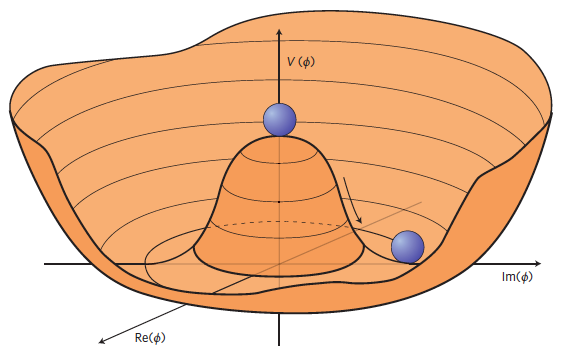
\includegraphics[width=0.97\textwidth]{figs/sm/higgspotential.png}
\caption{The potential of the Higgs field as a function of its real and imaginary components~\cite{Ellis:2013jnq}. The infinite number of degenerate ground states form a circle in phase space.}
\label{fig:higgsPotential}
\end{center}
\end{figure}

Through the spontaneous symmetry breaking of the Higgs potential, three of the four degrees of freedom of the Higgs field couple to and provide mass terms for the weak gauge bosons.
The remaining degree of freedom manifests as a single massive scalar field excitatation known as the \emph{Higgs boson}~\cite{Cheng:1985bj}.
Both the CMS and ATLAS experiments at CERN have independently confirmed the existence of a Higgs boson with a mass of $125 \pm 0.24 \GeV$~\cite{HiggsCMS,HiggsATLAS}. 

While the introduction of a Higgs field was motivated to explain the broken electroweak symmetry, it has allowed for of gauge invariant \emph{Yukawa} mass terms for fermions to be added to the SM Lagrangian.
In these terms, the strength of a fermion's Yukawa coupling to the Higgs results in the fermions gaining a non-zero mass~\cite{Cheng:1985bj}.
The experimental evidence for the Higgs coupling to fermions include the recent observations of \ttH~production~\cite{Sirunyan:2018hoz} and of the Higgs boson decaying a $\tau \overline{\tau}$ pair~\cite{CERN-EP-2018-221} and $b \overline{b}$ pairs~\cite{Sirunyan:2017guj}.

\subsection{Quantum Chromodynamics}\label{subsec:QCD}
The strong force and its interactions is described by Quantum Chromodynamics (QCD).
QCD is based on the non-Abelian $SU(3)_{colour}$ gauge group, which describes strong interactions through eight massless spin-$1$ gauge bosons called \emph{gluons} that act upon the \emph{colour} charge, \emph{C}, carried by quarks~\cite{ElectroweakStrong}.
Quarks carry either a red, green or blue colour charge, with anti-quarks possessing equivalent anti-colour charges.
Given the non-Abelian nature of QCD, gluons can self-couple as they themselves carry both a colour and and anti-colour charge, unlike the photon, for example, which is electrically neutral.

The self-coupling nature of gluons results in the phenomenon known as \emph{asymptotic freedom}~\cite{ElectroweakStrong,coughlan2006ideas,devenish2004deep}, whereby the strength of the strong coupling constant, $\alpha_{s}$, decreases with decreasing distance (increasing momenta).
This occurs as, like the QED vacuum of a sea of virtual $e^{+}e^{-}$ pairs, QCD considers the vacuum to be occupied by a virtual \emph{sea} of gluons and $q\overline{q}$ pairs.
In contrast to photons in QED however, as gluons self-couple, the virtual gluons have an attractive effect greater than the screening effect of virtual $q\overline{q}$ pairs.
Therefore, while $\alpha_{s}$ is sufficiently small inside a hadron for partons to behave as free particles, increasingly large amounts of energy are required to pull a hadron apart.
This results in the \emph{colour confinement} of partons~\cite{ElectroweakStrong,Griffiths,devenish2004deep}.
This behaviour of $\alpha_{s}$ means that when partons are liberated from hadrons, such as in the high energy hadron collisions of the LHC, the resultant shower of partons form new hadrons in a process known as hadronisation~\cite{Andersson:1983ia}.

In QED, the contribution to the calculation of the Matrix Element for a process decreases with increasing order of the diagram considered due to the electromagnetic coupling constant being considerably smaller than one.
In contrast however, higher order contributions in QCD become increasingly important as $\alpha_{s}$ increases, making higher order QCD calculations more and more difficult to perform.
It has been demonstrated that QCD calculations can be temporally split (factorised) into components that describe the long and short distance behaviours.
This allows the short distance components to be described using perturbation theory, such as the hard scattering of hadrons, while the long distance components are described using non-perturbative phenomenological models, such as Parton Distribution Functions (PDFs).
For a given hadron, PDFs describe the number density of each parton flavour as a function of the fraction of the hadron's momentum (Bjorken $x$) at a given energy scale.
PDFs are constrained by fits made to measurements made by a variety of different experiments~\cite{Ball:2014uwa,devenish2004deep}.
Figure~\ref{fig:pdf} shows the results of one the fit known as NNPDF3.0 which was used for the generation of the simulation samples considered in this thesis~\cite{Ball:2014uwa}.

\begin{figure}[htb]
\begin{center}
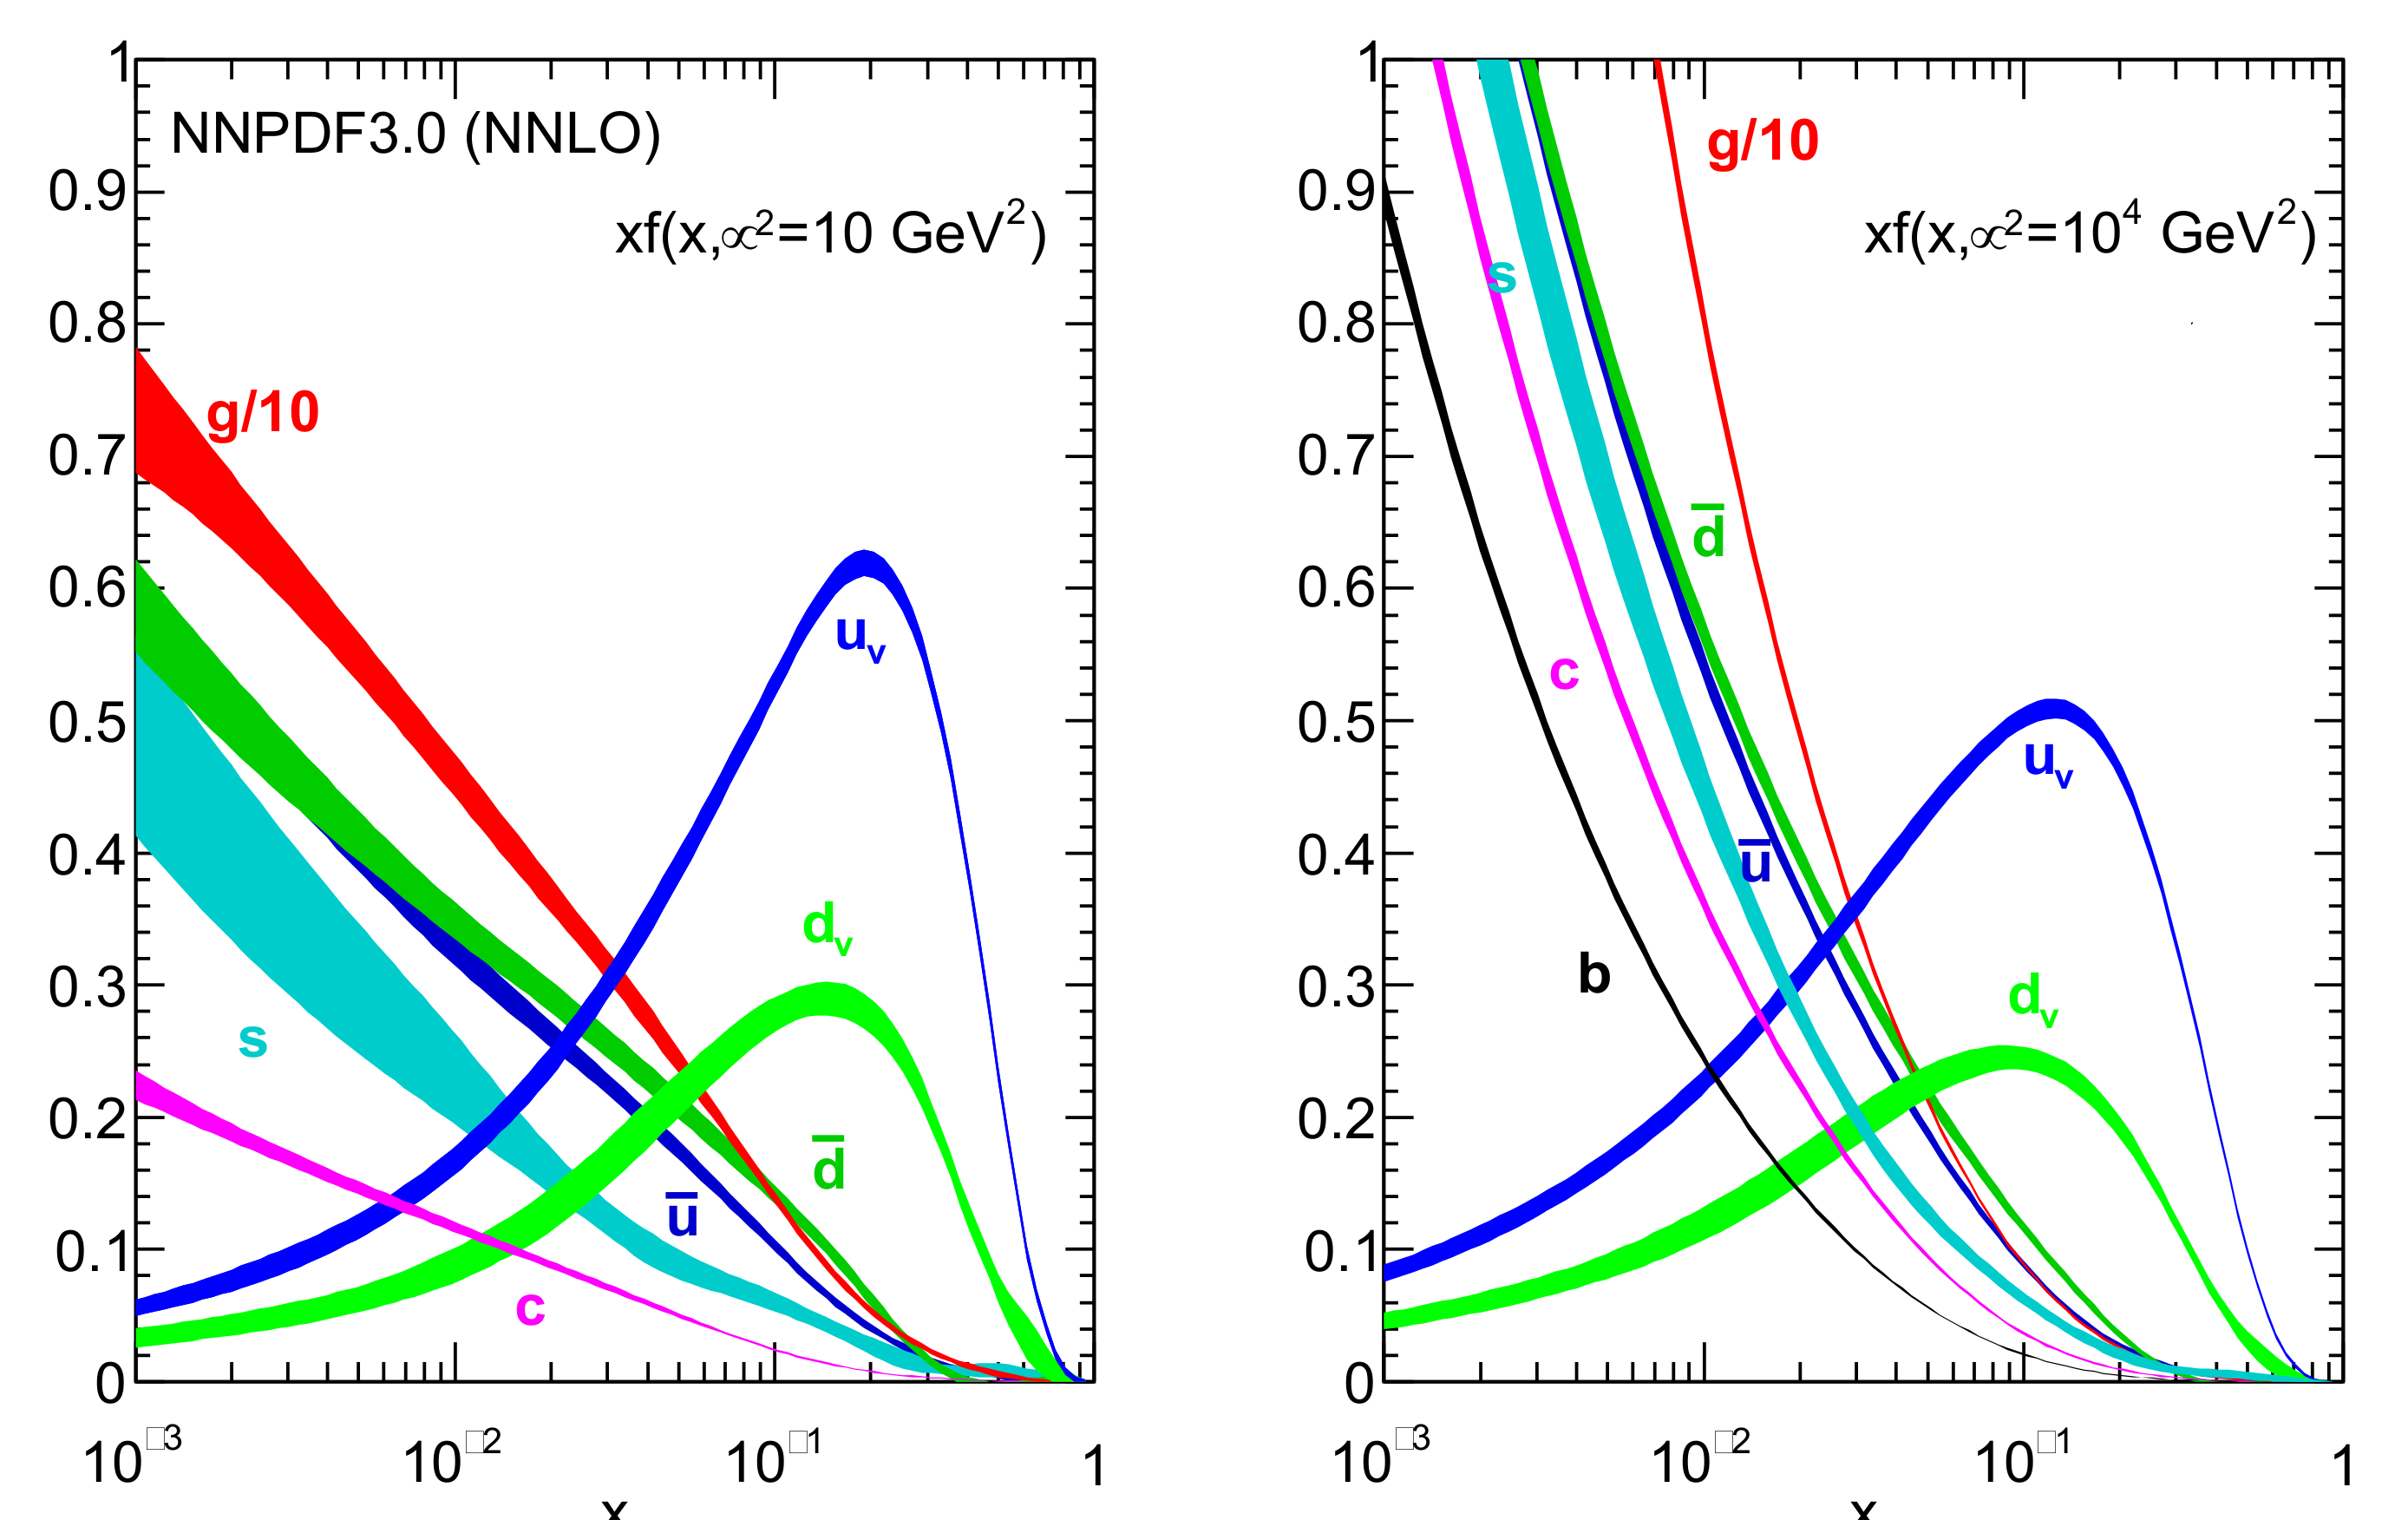
\includegraphics[width=0.97\textwidth]{figs/sm/pdf.png}
\caption{The proton parton distribution functions $xf(x)$ as a function of the momentum fraction determined by the NNPDF3.0 fit for factorisation scales of $\mu_{F} = 10\GeV^{2}$ (left) and $\mu_{F} = 10^{4}\GeV^{2}$~\cite{Ball:2014uwa}.
}
\label{fig:pdf}
\end{center}
\end{figure}

\section{Top Physics}\label{sec:top-physics}
The existence of a third generation of quarks was first hypothesised in 1973 by Makoto Kobayashi and Toshihide Maskawa as the CP violation observed in kaon decays was not possible with only two generations of quarks~\cite{Kobayashi:1973fv}.
This hypothesis was reinforced with the discovery of a third generation (tau) lepton in 1975 and a third generation down-type (bottom) quark in 1977~\cite{Herb:1977ek}, which strongly implied the existence of a weak isospin partner to the bottom quark.
As the top quark was more massive than initially assumed, it would remain unobserved until a sufficiently powerful collider was built.
Finally in 1995 the top quark was observed at the Tevatron at the Fermi National Accelerator Laboratory by the CDF and D\O\xspace experiments~\cite{Abe:1995hr,D0:1995jca}.

The top quark's mass, $m_{top}$, of $173.0 \pm 0.4 \GeV$~\cite{Tanabashi:2018oca} makes it the most massive known fundamental particle and is responsible for imbuing it with properties that have no equivalent for the other five quarks~\cite{Tanabashi:2018oca}.
Unlike the other five quarks, the top quark is massive enough to decay into an on-shell W boson, giving it a much shorter lifetime than the other quarks.
This lifespan of $5 \times 10^{-25}$ seconds is several orders of magnitude smaller than the characteristic timescale of the strong interaction~\cite{Quadt}.
Consequently, the top quark is the only quark that decays before it can hadronise, making it a unique probe into the nature of a ``bare'' quark, such as its spin and polarisation, through studying the angular distributions of its decay products~\cite{Khachatryan:2015dzz}.
This also makes it possible to determine the helicity of the W boson involved in the decay.
Measurements of the Wtb vertex allows for the $\abs{V_{tb}}$ element of the Cabibbo-Kobayashi-Maskawa (CKM) matrix to be directly measured and thus test whether the CKM matrix is unitary, as presumed, or otherwise~\cite{Shibata:2008sy}.

The top quark predominantly decays into a bottom quark and a W boson, as shown in Figure~\ref{fig:topDecay}.
Currently, the most precise measurement of the branching ratio for this decay mode has been measured to be $1.014 \pm 0.003 \textrm{(stat)} \pm 0.032 \textrm{(syst)}$ by the CMS Collaboration~\cite{Khachatryan:2014nda}.

\begin{figure}[htbp]
\begin{center}
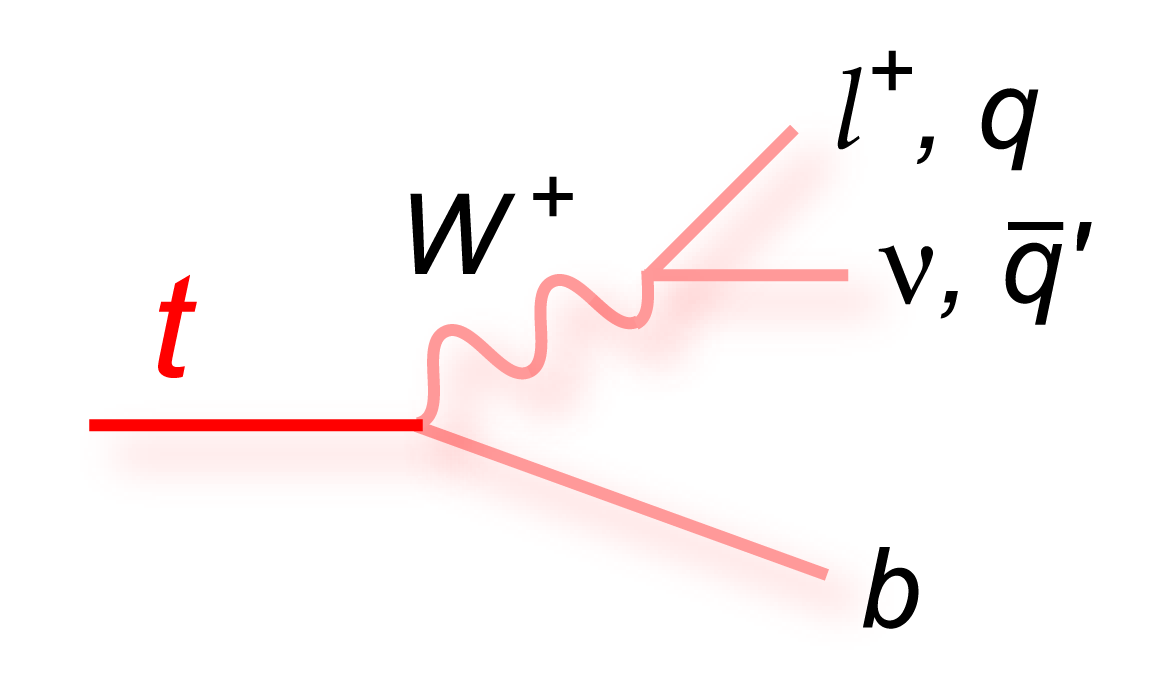
\includegraphics[width=0.57\textwidth]{figs/top-physics/topDecay.png}
\caption{The main decay mode of the top quark into a b-quark and W boson, where the W boson decays either leptonically or hadronically~\cite{topDiagrams}.}
\label{fig:topDecay}
\end{center}
\end{figure}

Given all these properties, the top quark makes an excellent probe of the Wtb vertex and is sensitive to any anomalous couplings that would impact it.
Additionally, with the top mass being greater than that of any other fundamental particle, it has the strongest Yukawa coupling to the Higgs field.
Consequently, many believe that the top quark has a special role to play in electroweak symmetry breaking and Beyond the Standard Model (BSM) Physics~\cite{Giammanco:2017xyn}
 
%The top quark has not been studied to the same extent as the other quarks due to its later discovery and the relatively low top quark production rate at the Tevatron limiting statistics.
%The greater operational energy and integrated luminosity provided by the LHC however, has produced greater statistics will be available to probe the nature of the top quark~\cite{Shibata:2008sy}. 

\subsection{Top quark pair production}\label{subsec:ttbarTheory}
At hadron colliders, top quarks are predominantly produced by pair production (\ttbar) through strong interactions.
As illustrated in the Feynman diagrams in figure~\ref{fig:feyn_ttbar}, at Leading Order (LO) \ttbar events are produced by either gluon fusion or quark-anti-quark annihilation. 
While approximately 85\% of \ttbar events produced at the Tevatron occured via quark fusion, 80-90\% of \ttbar events at the LHC are produced by gluon fusion for $\sqrt{s} = 8-14\TeV$~\cite{Tanabashi:2018oca,Deliot:2011np}.
These differences in production rates occur for two reasons:
\begin{itemize}
\item Higher centre-of-mass energies results in smaller Bjorken $x$, resulting in a much larger fraction of the proton's energy being carried by gluons.
\item The Tevatron was a proton-anti-proton collider, both quarks involved in quark fusion could be valance quarks, unlike the LHC where one would have to be a sea quark. 
\end{itemize} 

\begin{figure}[htbp]
\begin{center}
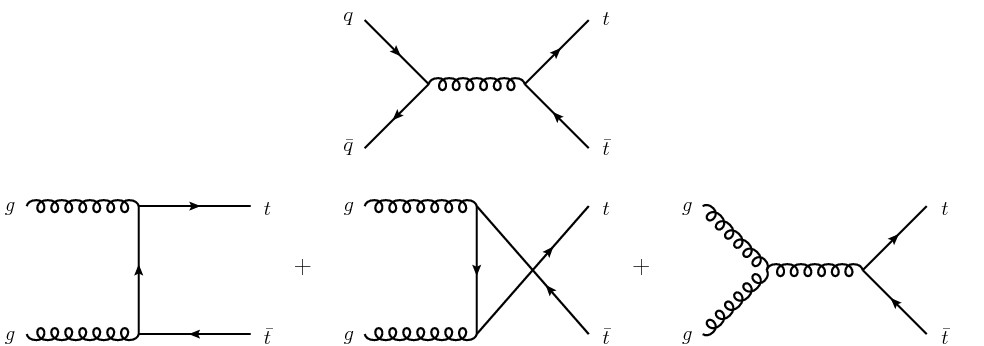
\includegraphics[width=0.97\textwidth]{figs/top-physics/ttbar_feyn.jpg}
\caption{The three Leading Order Feynman diagrams for top quark pair production at hadron colliders. Quark-anti-quark annihilation is illustrated on the top row and gluon fusion on the bottom.}
\label{fig:feyn_ttbar}
\end{center}
\end{figure}

As the top quark predominately decays into a W boson and a b-quark, the three different decay modes of pair produced top quarks are characterised by the manner in which the two W bosons decay:
\begin{itemize}
\item \textbf{hadronic} decays occur when both W bosons decay into a quark and anti-quark.
\item \textbf{lepton + jets} decays occur when one W boson decays into a lepton and its associated anti-neutrino, while the other W boson decays hadronically.
\item \textbf{dilepton} decays occur when both W bosons decay into a lepton and its associated anti-neutrino.
\end{itemize}
 

Top quark pair production can also occur in association with a vector boson (\ttV), albeit at relatively small cross sections compared to both \ttbar and single top production (see Section~\ref{subsec:tZqTheory}).
%Despite the relatively small production cross sections for \ttV processes, it is important that they are well understood as they form some of the irreducible background processes for other rare processes, such as tHq and tZq production~\cite{Khachatryan:2014ewa}.

\subsection{Single top quark production}\label{subsec:singleTopTheory}
Top quarks can also be produced singly through weak interactions, albeit with smaller cross sections than that for \ttbar production given the relative weakness of the electroweak coupling compared to the strong coupling.

There are three main SM single top production mechanisms, which are categorised by the virtuality of the W boson involved in the interaction.

\begin{figure}[htbp]
\centering
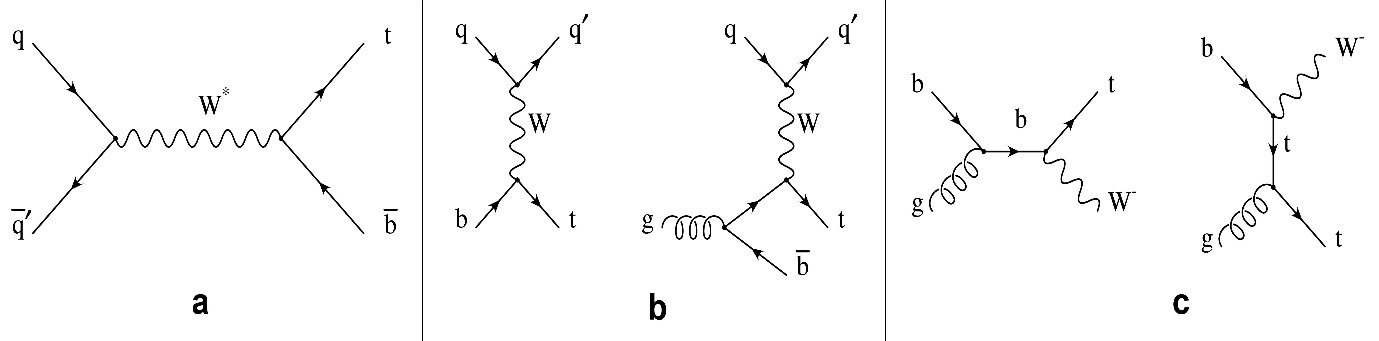
\includegraphics[width=1.00\textwidth]{figs/top-physics/singletop_feyn.jpg}
\caption{The leading order diagrams for each of the three single top production mechanisms: (a) s-channel, (b) t-channel and (c) single top production in association with a W boson (tW production).}
\label{fig:singleTopDiagrams}
\end{figure}

Figure~\ref{fig:singleTopDiagrams}(a) shows the first of these mechanisms, which is known as s-channel production. 
This is quark-anti-quark annihilation producing an off-shell W boson that decays into a top and anti-b quark.
This process has the lowest production cross section of the three at the LHC due to the charge-asymmetric initial state.
Given its low cross section and a final state topology similar to larger background processes, the s-channel has yet to be observed at the LHC~\cite{Khachatryan:2016ewo}.

The t-channel production mechanism, as shown in Figure~\ref{fig:singleTopDiagrams}(b), is the dominant single top prodution mechanism at the LHC.
The process involves the scattering of a W boson off a sea b quark or produced a b quark produced by gluon splitting.
Initially observed at the Tevatron~\cite{Aaltonen:2009jj,Abazov:2009ii}, the t-channel process has since been studied at higher energies at the LHC, with all results to date remaining consistent with the SM~\cite{Berta:2017ghf,Morton:2018wkb}.	

The tW production mechanism, as shown in Figure~\ref{fig:singleTopDiagrams}(c), is the process in which  a top quark is produced in association with an on-shell W boson.
In contrast to being negligible at the Tevatron, tW production is observable at the LHC and was discovered in 2014~\cite{Chatrchyan:2014tua}.

Single top production processes are a powerful probe of the electroweak interactions of the top quark.
In contrast to \ttbar, these processes allow for the Wtb vertex involved in top quark production to be probed in addition to providing complimentary measurements of the Wtb vertex in top quark decays.

Understanding single top quark production processes is also important from an experimental viewpoint as:
\begin{itemize}
\item These processes form backgrounds for not only SM processes such as \ttbar, but also for Higgs and BSM physics searches, such those which introduce new electroweak couplings.
\item Precision measurements of these processes can be used to compliment measurements of \ttbar processes in constraining Parton Distribution Functions~\cite{Guffanti:2010yu}.
\end{itemize}


\subsection{Single top production in association with a Z boson}\label{subsec:tZqTheory}
The analysis presented in this thesis is the search for the production of a single top quark in association with a Z boson with an additional jet, known as \emph{tZq} production, using the dilepton final state.

The high centre-of-mass energies and integrated luminosities available at the LHC have made it possible to not only perform precision studies of \ttbar and single top quark process, but also to make measurements of processes involving the tZ vertex.
Such measurements provide not only the ability to perform precision tests of SM predictions, but are also sensitive to new physics such as the existence of new electroweak bosons, new fermions or Flavour Changing Neutral Currents (FCNC).

\begin{figure}[htbp]
\centering
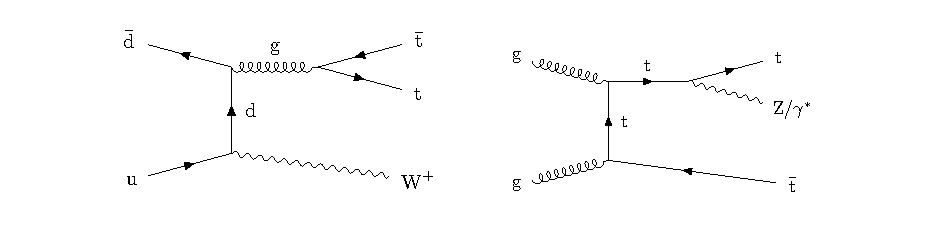
\includegraphics[width=\textwidth]{figs/top-physics/CMS-TOP-17-005_Figure_001.pdf}
\caption{Leading order \ttW~(left) and \ttZ~(right) production diagrams~\cite{Sirunyan:2017uzs}. Unlike \ttZ~and \ttH~production, the gauge boson in \ttW~is not radiated from the top quark, but from the initial state quarks.}
\label{fig:feyn_ttV}
\end{figure}

It may initially assumed that given the larger production cross section for \ttbar compared to single top processes that \ttbar processes would provide the best conditions to probe the electroweak interactions with the top quark.
The tW coupling however, can only be probed through the single top tW process as the W boson couples to the initial state quarks for \ttW~processes, as illustrated in figure~\ref{fig:feyn_ttV}.
tH has yet to be observed~\cite{CMS:2018jsz} as it is much more difficult to access than \ttH~due to the destructive interference between the tH and HW vertices~\cite{Maltoni:2001hu}.

%CMS has made measurements of \ttH, \ttW, and production, all of which are consistent with the corresponding SM predictions~\cite{Sirunyan:2017uzs,Sirunyan:2018hoz}.

In contrast,~\ttZ~has a lower production cross section than the combined tZ and $\overline{\text{t}}$Z production cross sections~\cite{Campbell:2013yla} as tZq contains fewer particles in the final state and thus is easier to produce.
CMS has made measurements of \ttH, \ttW, and \ttZ, all with signifiances in excess of five standard deviations and consistent with their SM predictions~\cite{Sirunyan:2018hoz,Sirunyan:2017uzs}.

tZq production is a rare SM process where a single top quark is produced in association with a Z boson with an additional jet.
Unlike \ttZ~where the Z boson is radiated from one of the top quarks, tZq involves the Z boson being radiated off one of the quark legs, as shown in the top two rows of Figure~\ref{fig:feyn_tZq}, or from the exchanged W boson, as shown shown in the bottom left diagram in Figure~\ref{fig:feyn_tZq}.
As tZq production is sensitive the WWZ coupling, unlike \ttZ~production, and is expected to be as sensitive to this coupling as WZ production, this process provides a unique precision probe of electroweak interactions with the top quark~\cite{Campbell:2013yla}.

In addition, tZq production needs to be well understood as it forms one of the irreducible backgrounds for other rare SM processes, such as tH production, as well as BSM processes such as Flavour Changing Neutral Currents (FCNC)~\cite{AguilarSaavedra:2004wm}.

\begin{figure}[h]
\centering
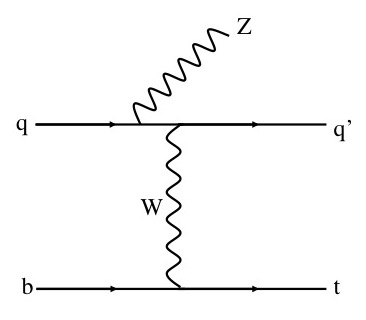
\includegraphics[width=0.37\textwidth]{figs/top-physics/tZq_feyn1.jpg}
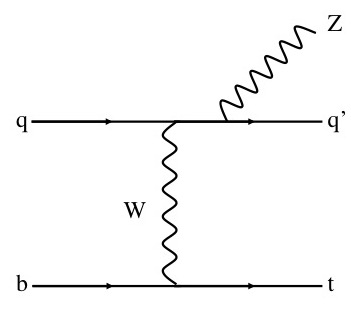
\includegraphics[width=0.37\textwidth]{figs/top-physics/tZq_feyn2.jpg}
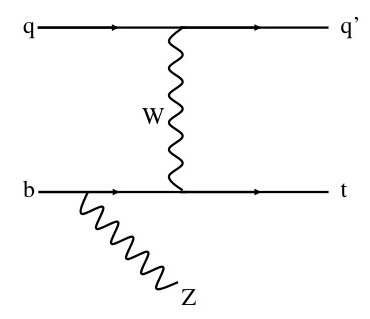
\includegraphics[width=0.37\textwidth]{figs/top-physics/tZq_feyn3.jpg}
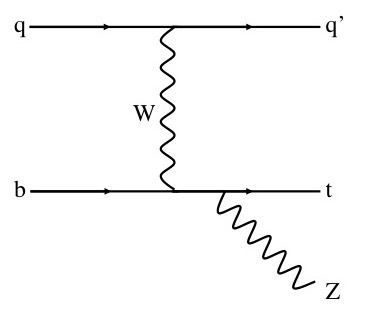
\includegraphics[width=0.37\textwidth]{figs/top-physics/tZq_feyn4.jpg}
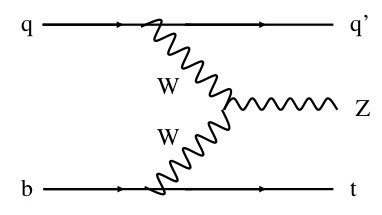
\includegraphics[width=0.37\textwidth]{figs/top-physics/tZq_feyn5.jpg}
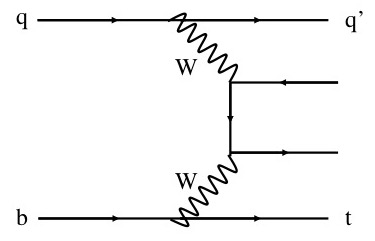
\includegraphics[width=0.37\textwidth]{figs/top-physics/tZq_feyn6.jpg}
\caption{Leading order tZq production diagrams, where the Z boson is radiated off one of the quark lines in the diagrams in the top two rows, where the Z boson is radiated off the exchanged W in the lower left diagram and from the non-resonant contribution to the tZq process in the bottom right diagram.}
\label{fig:feyn_tZq}
\end{figure}

As the top quark predominately decays into a W boson and a b-quark, the four possible final states are characterised by the decay mode of the Z boson and W boson:
\begin{itemize}
\item \textbf{trilepton:} when the W boson decays into a lepton and neutrino and the Z boson decays into a lepton and anti-lepton.
\item \textbf{dilepton:} when the Z boson decays into a pair of leptons and the W boson into a quark and anti-quark. 
\item \textbf{single lepton:} where the W boson decays into a lepton and neutrino and the Z boson decays into a quark and anti-quark.
\item \textbf{hadronic:} both the W boson and Z boson decay into a quark and anti-quark.
\end{itemize}

The physics analysis presented in this thesis is the first search at CMS for tZq using the dilepton final state.
The initial searches for tZq however, used the trilepton final state, as while it has a smaller production cross section than either of the dilepton or hadronic final states, it is the easiest to distinguish against background processes.

The first search for tZq however, was unable to observe the process, making a measurement with an observed significance of 2.9 $\sigma$~\cite{Sirunyan:2017kkr}.
Both ATLAS and CMS have since been able to observe the trilepton final state for tZq at $\sqrt{s} = 13\TeV$ as a result of the tZ and $\overline{\text{t}}$Z cross sections increasing with the centre-of-mass energy at a similar rate to \ttZ~and the large integrated luminosity delivered by the LHC at $\sqrt{s} = 13\TeV$~\cite{Aaboud:2017ylb,Sirunyan:2017nbr}.
This increase in the tZq production cross section and the large integrated luminosity being delivered by the LHC at $\sqrt{s} = 13\TeV$ has also made it possible to perform searches for the other tZq final states, including the dilepton final state, allowing for complimentary measurements of this process to be made.

The observed results presented in this work and the previous CMS searches for tZq using the trilepton final state at $\sqrt{s} = 13\TeV$ use the reference next-to-leading order production cross section for tZq where the Z boson decays leptonically, for $m_{ll} > 30 \GeV$~\cite{Sirunyan:2017nbr}:

\begin{equation}
\sigma ( \textrm{tZq}, Z \rightarrow l^{+} l^{-}) = 94.2^{+1.9}_{-1.8}\textrm{scale}\pm{2.5}\textrm{ (PDF) fb} \;
\label{tZqCrossSection}
\end{equation}

The analysis strategy and full event selection requirements used in the analysis of this process is discussed in detail in Chapter~\ref{chapter:tzq-search}, the modelling of the backgrounds in Chapter~\ref{chapter:bkg} and the statistical methodology used to perform the measurement of this process in Chapter~\ref{chapter:results}.

\section{Beyond the Standard Model Physics}\label{sec:bsm}
The SM has been incredibly successful at accurately predicting the majority of the properties of the known fundamental particles up to the electroweak scale.
However, given the inability of the SM to incorporate gravity and to fully address a number of experimental observations, such as massive neutrinos, it is apparent that there must be new physics beyond the Standard Model.

\subsection{Shortcomings of the Standard Model Physics}\label{subsec:shortcomings}
One of the major and most apparent shortcomings of the SM is its inability to explain why there is an asymmetry between matter and anti-matter in the universe.
While CP symmetry violation does occur within the SM, it is insufficient to account for the amount of matter observed in the universe.

Gravity is currently described by the extremely successful classical theory of General Relativity (GR).
GR however, is fundamentally incompatible with the SM and  has produced contradictory results, such as their predictions for the cosmological constant differing by 120 orders of magnitude~\cite{Adler:1995vd}.
While attempts have been made to reconcile the two theories, no successful quantum theory of gravity has yet been produced~\cite{Sola:2013gha}.	

One of the other serious theoretical issues with the SM is the \emph{hierarchy problem} concerning the lack of explanation for the vast differences observed between the electroweak scale and the Grand Unified Theory and Plank scales where gravity becomes strong~\cite{Burdman:2007ck}.
The mass of the Higgs boson presents a related hierarchy problem.
As the vacuum expectation value of the Higgs field determines the mass of the weak bosons, for the observed masses of these bosons, one would expect a vacuum expectation value of approximately 246\GeV.
Given that the radiative corrections to the observable mass of the Higgs boson are proportional to the energy scale of any new physics, this would imply that the Higgs vacuum expectation value would be either zero or of the order Plank's constant.
In order to obtain the observed Higgs mass of 125\GeV, the cancellations required from the radiative corrections must be extremely ``fine tuned''.
While there is nothing fundamentally wrong with this, many scientists find such fine tuning to be \emph{unnatural}.

%Other astronomical and cosmological inconsistencies include the presence of \emph{dark matter} (DM) and \emph{dark energy} in the universe.
%The observations of the rotation of galaxies, gravitational lensing, structure of the universe and the Cosmic Microwave background, indicates that there must be a form of ``dark'' matter present~\cite{Aghanim:2018eyx}.
%The accelerating expansion of the universe is also unaccounted for and implies the existence of a ``dark energy'' to drive this~\cite{Peebles:2002gy,Aghanim:2018eyx}.

Perhaps the greatest inconsistency experimentally observed with the SM is the fact that neutrinos are not massless.
The first indication of massive neutrinos was made by the Homestake experiment, which found that the fraction of electron neutrinos arriving from the Sun was at most half what was expected~\cite{PhysRevLett.20.1205}.
While this observation could be explained by neutrinos experiencing flavour oscillations, this would require neutrinos to have mass in contrast to the expectations of the SM in order for their flavour eigenstates to mix with their mass eigenstates.
Further experiments have confirmed however, that neutrinos do undergo flavour oscillations and thus must have mass~\cite{Fukuda:1998mi,Ahmad:2001an,PhysRevD.88.032002}.

%\subsection{Flavour Changing Neutral Currents}\label{sec:fcncs}
%Given the limited experimental evidence of BSM physics, a large number of BSM physics models, driven by theoretical and ascetic arguments, have been proposed to account for the shortcomings of the SM.
%While the analysis presented in this thesis concerns the search for a SM process, the tZq cross section is sensitive to modifications of the tZ coupling posited by a number of BSM theories.
%
%As eluded to in Section~\ref{subsec:weakForce}, any flavour changing process involving a neutral weak current in the SM cannot occur at the tree level and requires a loop processes involving a virtual W exchange.
%A number of BSM theories however, introduce top quark FCNC decay contributions at the tree level, such as Supersymmetry (SUSY) models and those proposing additional Higgs doublets and/or quark singlets~\cite{AguilarSaavedra:2004wm}.
%The presence of such new tZ couplings would enhance the production rate of both \ttZ and tZq by several orders of magnitude and should be observable at the LHC. 
%As of to date however, no evidence for BSM FCNCs have been observed for the tZ coupling for both single top and \ttbar processes~\cite{Sirunyan:2017kkr}.
